%-----------------------------------------------------------------------------------------------
\chapter{Algoritmusok, paraméterek}\label{sect:AlgPar}
%-----------------------------------------------------------------------------------------------

A strukturált fényt használó rekonstrukciós eljárások alapja, hogy előre ismert mintát vetítenek a fényképezett objektumra, majd ennek torzulásai alapján következtetnek a mélységinformációra.
A Kinect első verziója is így működik.
Az eszköz mélységképet szolgáltató része (kamera és projektor) az infravörös tartományban üzemel.
A vetített minta egy látszólag véletlenszerű\footnote{Valójában úgy tervezték a pontfelhőt, hogy minimális legyen az egy sorban lévő ismétlődő vagy hasonló blokkok száma} eloszlást követő pontfelhő.
A minta formális leírása vagy a generálás algoritmusa nem ismert, ezért a rekonstrukcióhoz elengedhetetlen valamilyen referenciakép készítése.
A diszparitás meghatározását ez némileg bonyolítja, extra feldolgozási lépéseket tesz szükségessé.

Az extra lépések oka, hogy jelentős időbeli különbség van a referencia- és adatkép készítése között.
Ez idő alatt szinte garantáltan változnak a fényviszonyok, amit kompenzálni kell.
A feladat megoldására 3 lépcsős feldolgozást valósítottam meg, amik a következőkben ismertetésre fognak kerülni.

A rekonstrukció mintaillesztésen alapuló \emph{diszparitás meghatározás}.
Az illeszkedés minőségének javítása érdekében szükség van \emph{előfeldolgozási lépésekre}.
Az diszparitáskép szűrésére és emberi fogyasztásra alkalmassá tételére pedig szükség van \emph{utófeldolgozásra}.

%-----------------------------------------------------------------------------------------------
\section{Előfeldolgozási lépések}\label{sect:Preproc}
%-----------------------------------------------------------------------------------------------

Az előfeldolgozás szükségességét a \figref{needToPreproc} ábra jól mutatja.
Ilyen mértékű fényerőkülönbség esetén a legtöbb mintaillesztési eljárás csődöt mondana.
A jelenség kiküszöbölésére több algoritmust is próbáltam a félév során, melyek változó mértékben voltak eredményesek.
A következőkben ismertetem a kipróbált feldolgozási lépéseket.

\begin{figure}[ht!]
	\begin{subfigure}{.5\textwidth}
	  \centering
	  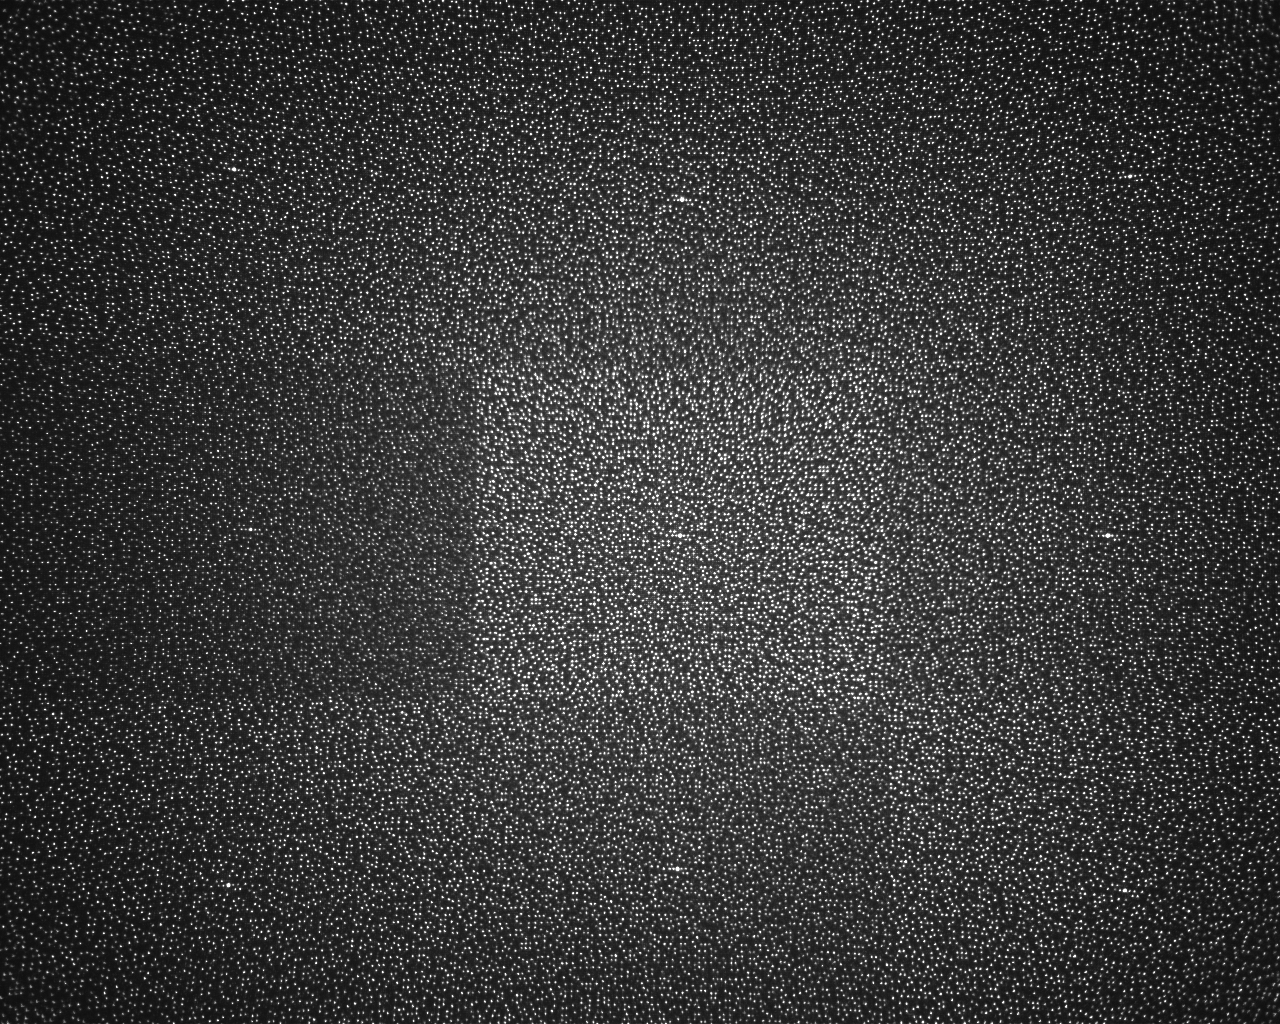
\includegraphics[width=0.9\linewidth]{figures/unproc_ref.png}
	  \caption{Nyers referencia kép}
	  \label{fig:unprocRef}
	\end{subfigure}
	\begin{subfigure}{.5\textwidth}
	  \centering
	  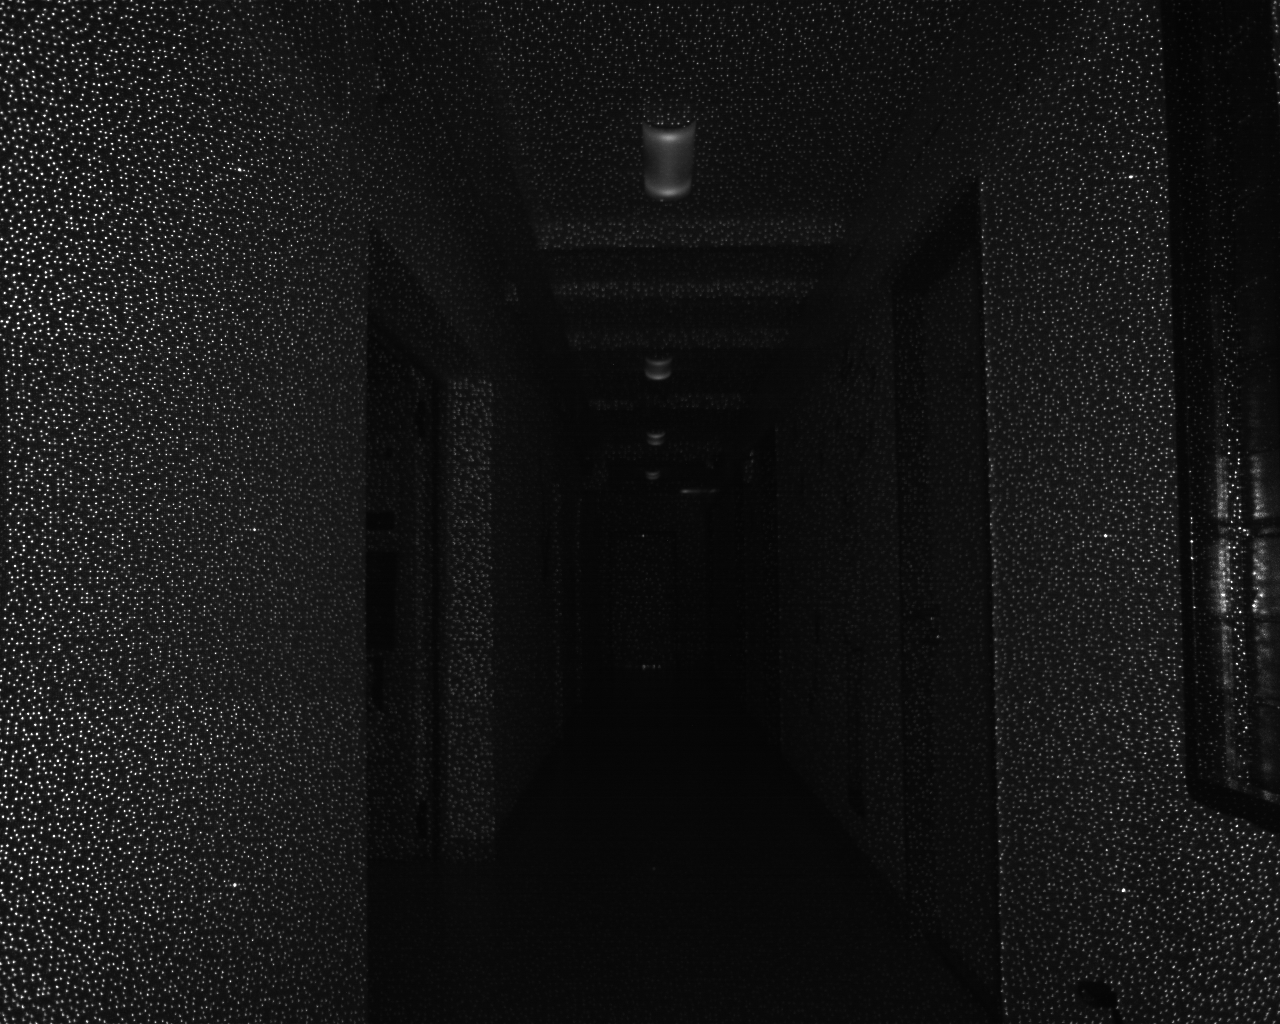
\includegraphics[width=0.9\linewidth]{figures/unproc_data.png}
	  \caption{Nyers adat kép}
	  \label{fig:unprocData}
	\end{subfigure}
	\caption{Fényviszonyok különbsége feldolgozás előtt}
	\label{fig:needToPreproc}
\end{figure}

%-----------------------------------------------------------------------------------------------
\subsection{Difference of Gaussians}\label{sect:DoG}
%-----------------------------------------------------------------------------------------------

Az első ígéretes irány a felüláteresztő szűrés volt.
Ennek egy lehetséges implementáció a DoG eljárás.

%-----------------------------------------------------------------------------------------------
\subsection{Hisztogram kiegyenlítés}\label{sect:histNorm}
%-----------------------------------------------------------------------------------------------

%-----------------------------------------------------------------------------------------------
\subsection{Egyéb előfeldolgozás}\label{sect:scale}
%-----------------------------------------------------------------------------------------------


%-----------------------------------------------------------------------------------------------
\section{Diszparitás meghatározás}\label{sect:Depthproc}
%-----------------------------------------------------------------------------------------------

%-----------------------------------------------------------------------------------------------
\section{Utófeldolgozás}\label{sect:Postproc}
%-----------------------------------------------------------------------------------------------


%-----------------------------------------------------------------------------------------------
\subsection{Medián szűrő}\label{sect:median}
%-----------------------------------------------------------------------------------------------


%-----------------------------------------------------------------------------------------------
\subsection{Vizualizáció}\label{sect:visual}
%-----------------------------------------------------------------------------------------------

